\chapter{Quantum Entanglements, Part 1}

We begin with a very specific puzzle: two entangled states of two spins differ only by a sign, and yet that sign changes the physics in an essential way. The lecture does not begin with a general theory of entanglement. It begins with that puzzle, rebuilds the computational machinery needed to answer it, and then follows the answer outward: first to the singlet and its perfect anti-correlation, then to Bell's inequality, and finally to the impossibility of universal quantum cloning. These notes follow Leonard Susskind's lecture closely, with curation by LazyingArt LLC.

\section{Sign Choice in the Two-Spin State}

Let us label the spin states of a single spin by
\[
|u\rangle,\qquad |d\rangle,
\]
with the understanding that these are eigenstates of the third component of spin. For two spins we suppress the tensor-product symbol and write, for example,
\[
|ud\rangle = |u\rangle_1\otimes |d\rangle_2.
\]

The lecture opens with the two superpositions
\begin{equation}
|\psi_{\pm}\rangle
=
\frac{|ud\rangle \pm |du\rangle}{\sqrt{2}}.
\end{equation}
In both of them the third components are opposite: whenever one spin is up along the \(3\)-axis, the other is down. At first sight the two states sound nearly identical. Each displays a sharp correlation in the third component. But the whole point of the lecture is that the sign is not cosmetic. We must ask what survives when we stop looking only at the third component.

Susskind inserts the normalization immediately. The \(\sqrt{2}\) is not decoration; it is what makes the two probabilities add to one. With that done, the real question is now sharp: what observable can actually distinguish the two states?

\section{Recalling the Pauli Actions and the Vanishing of One-Spin Averages}

Before answering that question, the lecture deliberately rewrites the elementary action table for the Pauli matrices. This is not a detour. It is the small computational engine that drives every later calculation.

\begin{figure}[h]
\centering

\includegraphics[width=0.44\textwidth]{lecture_05_figure_02.png}
\caption{First line of the Pauli-action table as it is restarted on the board.}
\end{figure}

We use
\begin{align}
\sigma_1|u\rangle &= |d\rangle, &
\sigma_1|d\rangle &= |u\rangle, \\
\sigma_2|u\rangle &= i|d\rangle, &
\sigma_2|d\rangle &= -i|u\rangle, \\
\sigma_3|u\rangle &= |u\rangle, &
\sigma_3|d\rangle &= -|d\rangle.
\end{align}
For the second spin we introduce an identical family of operators \(\tau_1,\tau_2,\tau_3\), acting on the second slot rather than the first.

Now comes the first perhaps surprising claim: for either sign choice, every one-spin expectation value vanishes,
\begin{equation}
\langle \sigma_i\rangle = 0,
\qquad
\langle \tau_i\rangle = 0.
\end{equation}
So neither individual spin is definitely polarized in any direction. The state of either constituent spin, taken by itself, carries no preferred axis.

\begin{figure}[h]
\centering

\includegraphics[width=0.58\textwidth]{lecture_05_figure_03.png}
\caption{Board layout for the entangled state and the vanishing one-spin expectation claim.}
\end{figure}

\paragraph{Worked check.}
For the explicit board calculation Susskind chooses the plus state and checks \(\sigma_3\):
\begin{align}
\langle \psi_+|\sigma_3|\psi_+\rangle
&=
\frac{1}{2}
(\langle ud|+\langle du|)\sigma_3(|ud\rangle+|du\rangle) \\
&=
\frac{1}{2}
(\langle ud|+\langle du|)(|ud\rangle-|du\rangle) \\
&=
\frac{1}{2}(1-1) \\
&= 0.
\end{align}
The cross terms vanish because \(\langle ud|du\rangle=\langle du|ud\rangle=0\).

\subsection{Question \& Answer}

\paragraph{Question.} Does \(\langle \sigma_i\rangle=0\) mean that the spin has eigenvalue \(0\)?

\paragraph{Answer.} No. For a single spin component the only measurement outcomes are \(\pm 1\). There is no eigenstate of \(\sigma_i\) with eigenvalue \(0\). What vanishes is the expectation value, not the individual outcome. In this state a measurement of a single component is a fair coin toss: up and down occur with equal probability.

This distinction matters. If one compresses it away, the entire first half of the lecture becomes misleading. The one-spin observables do not distinguish the two entangled states.

\section{Total Spin, Singlet, and EPR Correlation}

The decisive move is to stop looking at one spin at a time and instead look at the sum of the two spins. In the lecture this is motivated as the sum of two little magnetic moments. Mathematically the relevant operators are
\[
\sigma_1+\tau_1,\qquad
\sigma_2+\tau_2,\qquad
\sigma_3+\tau_3.
\]

We begin with the third component. On the basis states,
\begin{align}
(\sigma_3+\tau_3)|ud\rangle &= (1-1)|ud\rangle = 0, \\
(\sigma_3+\tau_3)|du\rangle &= (-1+1)|du\rangle = 0.
\end{align}
Therefore
\begin{equation}
(\sigma_3+\tau_3)(|ud\rangle \pm |du\rangle)=0.
\end{equation}
So both sign choices are eigenstates of \(\sigma_3+\tau_3\) with eigenvalue \(0\). This, by itself, does not yet distinguish them.

Now apply \(\sigma_1+\tau_1\). Using \(\sigma_1|u\rangle=|d\rangle\) and \(\sigma_1|d\rangle=|u\rangle\),
\begin{align}
(\sigma_1+\tau_1)|ud\rangle &= |dd\rangle + |uu\rangle, \\
(\sigma_1+\tau_1)|du\rangle &= |uu\rangle + |dd\rangle.
\end{align}
Hence
\begin{equation}
(\sigma_1+\tau_1)(|ud\rangle+|du\rangle)
=
2|uu\rangle+2|dd\rangle,
\end{equation}
while
\begin{equation}
(\sigma_1+\tau_1)(|ud\rangle-|du\rangle)=0.
\end{equation}
The sign has finally become physical. The plus state is not annihilated by \(\sigma_1+\tau_1\), but the minus state is.

The same pattern holds in the second direction. Using the \(\sigma_2\) and \(\tau_2\) action table, one finds
\begin{equation}
(\sigma_2+\tau_2)(|ud\rangle-|du\rangle)=0.
\end{equation}
Thus the minus-sign state is annihilated by all three components of the total spin operator. In compact form,
\begin{equation}
(\vec{\sigma}+\vec{\tau})\cdot \hat n\,|\psi_-\rangle=0
\qquad
\text{for every unit vector }\hat n.
\end{equation}

This is the state Susskind now singles out. It is the singlet state. The plus-sign state, by contrast, is the triplet combination relevant to this two-dimensional subspace.

The payoff is immediate. In the singlet, if one observer measures any component of one spin, the other observer knows with certainty what the corresponding component of the other spin will be: it must be the opposite value, because the sum is always zero. This is the EPR-type correlation that drives the rest of the lecture.

\subsection{Question \& Answer}

\paragraph{Question.} Is this only true on average, or is it true every single time?

\paragraph{Answer.} Every single time, provided we are talking about the singlet and the same component of spin on both particles. The reason is not merely statistical. The singlet is an eigenvector of the total spin operator in every direction, with eigenvalue \(0\). For an eigenvector, repeated measurements of that observable yield the eigenvalue with certainty.

\subsection{Question \& Answer}

\paragraph{Question.} Do these correlations violate causality, or let Alice and Bob signal faster than light?

\paragraph{Answer.} No. Bob's measurement lets Bob infer what Alice would get if she measured the same component, but Alice learns nothing new unless Bob sends her an ordinary classical message. Her local statistics remain fifty-fifty. No usable information is transmitted by the correlation alone.

\section{Bell's Inequality as a Classical Statement About Sets}

Having established the singlet and its correlation structure, the lecture deliberately resets. Bell's inequality is introduced as a theorem of ordinary classical logic, before any quantum mechanics is used.

Let a classical ensemble consist of objects that may or may not possess three properties \(A\), \(B\), and \(C\). We write \(N(A,\neg B)\) for the number of objects that have property \(A\) and do not have property \(B\). Bell's inequality is
\begin{equation}
N(A,\neg B)+N(B,\neg C)\ge N(A,\neg C).
\end{equation}

Susskind wants this proved by a picture, not by metaphysical commentary. The content is entirely classical.

\begin{figure}[h]
\centering
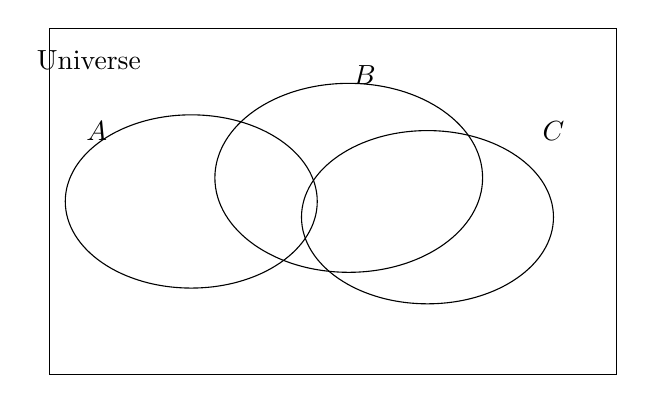
\begin{tikzpicture}[scale=1.0]
\draw (-3.6,-2.2) rectangle (3.6,2.2);
\node at (-3.1,1.8) {Universe};
\draw (-1.8,0.0) ellipse (1.6 and 1.1);
\draw (0.2,0.3) ellipse (1.7 and 1.2);
\draw (1.2,-0.2) ellipse (1.6 and 1.1);
\node at (-3.0,0.9) {$A$};
\node at (0.4,1.6) {$B$};
\node at (2.8,0.9) {$C$};
\end{tikzpicture}
\caption{A classical picture of three properties as subsets of a set.}
\end{figure}

A clean proof is this: every object counted by \(A\wedge \neg C\) either has \(B\) or does not have \(B\). If it does not have \(B\), then it lies in \(A\wedge \neg B\). If it does have \(B\), then because it also has \(\neg C\), it lies in \(B\wedge \neg C\). Therefore
\[
A\wedge \neg C \subset (A\wedge \neg B)\cup(B\wedge \neg C),
\]
and taking cardinalities gives the inequality.

Nothing quantum has happened yet. This is a theorem about subsets of a set.

\section{From Spin Propositions to Projection Operators}

Now the lecture translates the abstract symbols \(A,B,C\) into propositions about the singlet pair. We take
\begin{align}
A &: \text{spin 1 is up at }0^\circ \text{, i.e. along the }3\text{-axis}, \\
B &: \text{spin 1 is up at }45^\circ \text{ in the }zx\text{-plane}, \\
C &: \text{spin 1 is up at }90^\circ \text{ in the same plane}.
\end{align}

\begin{figure}[h]
\centering
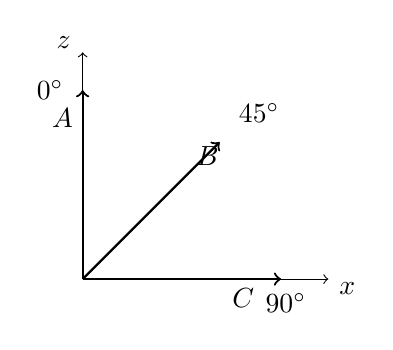
\begin{tikzpicture}[scale=1.2]
\draw[->] (0,0)--(0,2.4);
\draw[->] (0,0)--(2.6,0);
\node at (-0.2,2.5) {$z$};
\node at (2.8,-0.1) {$x$};
\draw[thick,->] (0,0)--(0,2.0);
\draw[thick,->] (0,0)--(1.45,1.45);
\draw[thick,->] (0,0)--(2.1,0);
\node[left] at (0,1.7) {$A$};
\node[above right] at (1.1,1.1) {$B$};
\node[below] at (1.7,0) {$C$};
\node[left] at (-0.1,2.0) {$0^\circ$};
\node[above right] at (1.55,1.55) {$45^\circ$};
\node[below] at (2.15,-0.05) {$90^\circ$};
\end{tikzpicture}
\caption{The \(0^\circ\), \(45^\circ\), and \(90^\circ\) directions used in the Bell discussion.}
\end{figure}

Because we are in the singlet, the negation of a statement about spin 1 can be converted into a positive statement about spin 2. Thus \(\neg B\) becomes the statement that spin 2 is up at \(45^\circ\), and \(\neg C\) becomes the statement that spin 2 is up at \(90^\circ\).

At this point the lecture asks the practical question: how are we to compute the relevant probabilities? That is what motivates projection operators.

\begin{figure}[h]
\centering

\includegraphics[width=0.58\textwidth]{lecture_05_figure_04.png}
\caption{Projection operator notation on the board, together with the geometric picture of projection onto a subspace.}
\end{figure}

We write, in standard form,
\begin{equation}
P|\alpha\rangle = |\alpha_p\rangle,
\end{equation}
meaning that \(P\) projects the vector \(|\alpha\rangle\) onto the chosen subspace. The board notation is partially obscured, but the geometric intent is clear and matches the standard construction.

\begin{figure}[h]
\centering
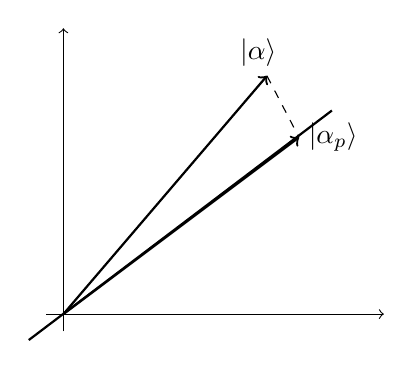
\begin{tikzpicture}[scale=1.1]
\draw[->] (-0.2,0)--(3.7,0);
\draw[->] (0,-0.2)--(0,3.3);
\draw[thick] (-0.4,-0.3)--(3.1,2.35);
\draw[->,thick] (0,0)--(2.35,2.75);
\node[above] at (2.25,2.75) {$|\alpha\rangle$};
\draw[dashed] (2.35,2.75)--(2.72,2.04);
\draw[->,thick] (0,0)--(2.72,2.04);
\node[right] at (2.72,2.04) {$|\alpha_p\rangle$};
\end{tikzpicture}
\caption{A clean redraw of the projection geometry used in the lecture.}
\end{figure}

For a single spin, the projection onto the \(\sigma_3=+1\) subspace simply removes the down component.

\begin{figure}[h]
\centering

\includegraphics[width=0.58\textwidth]{lecture_05_figure_05.png}
\caption{Projection operators acting on a general spinor, and the move to their matrix form.}
\end{figure}

Thus
\begin{equation}
P_{\sigma_3=+1}
\begin{pmatrix}
\alpha \\ \beta
\end{pmatrix}
=
\begin{pmatrix}
\alpha \\ 0
\end{pmatrix},
\qquad
P_{\sigma_3=-1}
\begin{pmatrix}
\alpha \\ \beta
\end{pmatrix}
=
\begin{pmatrix}
0 \\ \beta
\end{pmatrix}.
\end{equation}
The corresponding matrix is
\begin{equation}
P_{\sigma_3=+1}
=
\begin{pmatrix}
1 & 0 \\
0 & 0
\end{pmatrix}
=
\frac{1+\sigma_3}{2}.
\end{equation}
Likewise,
\begin{equation}
P_{\sigma\cdot \hat n = +1}
=
\frac{1+\sigma\cdot \hat n}{2}.
\end{equation}

The lecture then recasts the probability postulate in projector language:
\begin{equation}
\mathrm{Prob}(\alpha\text{ true in state }|\psi\rangle)
=
\langle \psi|P_\alpha|\psi\rangle.
\end{equation}

For the Bell quantity \(A\wedge \neg B\), the corresponding projector is
\begin{equation}
P_{A\wedge \neg B}
=
\frac{1+\sigma_3}{2}\,
\frac{1+\tau\cdot \hat n_{45}}{2},
\qquad
\hat n_{45}=\frac{\hat x+\hat z}{\sqrt{2}},
\qquad
\tau\cdot \hat n_{45}
=
\frac{\tau_1+\tau_3}{\sqrt{2}}.
\end{equation}

\subsection{Question \& Answer}

\paragraph{Question.} Why does the product of projectors represent the logical word ``and''?

\paragraph{Answer.} Only when the projectors commute. For a single electron, asking whether the spin is up along the \(3\)-axis and up along the \(1\)-axis is not a meaningful joint proposition, because the corresponding projectors do not commute. Here, however, one projector acts on spin 1 and the other on spin 2, so the \(\sigma\)'s commute with the \(\tau\)'s. In that compatible case the product does represent the conjunction of the two statements.

\section{Quantum Violation of Bell's Inequality}

Now the lecture does the calculation. Let
\begin{equation}
|\psi_s\rangle
=
\frac{|ud\rangle-|du\rangle}{\sqrt{2}}
\end{equation}
denote the singlet.

\paragraph{First probability: \(P(A,\neg B)\).}
We calculate
\[
P(A,\neg B)=\langle \psi_s|P_{A\wedge \neg B}|\psi_s\rangle.
\]
Act first with the projector \((1+\sigma_3)/2\). It kills the \(|du\rangle\) piece and leaves
\[
\frac{1}{\sqrt{2}}|ud\rangle.
\]
Now apply the second projector:
\begin{align}
\frac{1+\tau\cdot \hat n_{45}}{2}|ud\rangle
&=
\frac{1}{2}
\left(
|ud\rangle
+
\frac{\tau_1+\tau_3}{\sqrt{2}}|ud\rangle
\right) \\
&=
\frac{1}{2}
\left(
|ud\rangle
+
\frac{|uu\rangle-|ud\rangle}{\sqrt{2}}
\right) \\
&=
\frac{1}{2}
\left(
\left(1-\frac{1}{\sqrt{2}}\right)|ud\rangle
+
\frac{1}{\sqrt{2}}|uu\rangle
\right).
\end{align}
When we take the inner product with \(\langle\psi_s|\), the \(|uu\rangle\) term drops out because it is orthogonal to both \(\langle ud|\) and \(\langle du|\). Therefore
\begin{equation}
P(A,\neg B)
=
\frac{1}{4}\left(1-\frac{1}{\sqrt{2}}\right).
\end{equation}

By rotational invariance of the singlet,
\begin{equation}
P(B,\neg C)
=
\frac{1}{4}\left(1-\frac{1}{\sqrt{2}}\right).
\end{equation}

\paragraph{Second probability: \(P(A,\neg C)\).}
Now \(\neg C\) becomes ``spin 2 up at \(90^\circ\),''
so the relevant projector is
\[
\frac{1+\sigma_3}{2}\,\frac{1+\tau_1}{2}.
\]
Again \((1+\sigma_3)/2\) kills \(|du\rangle\), leaving \(|ud\rangle/\sqrt{2}\). Then
\[
\frac{1+\tau_1}{2}|ud\rangle
=
\frac{1}{2}(|ud\rangle+|uu\rangle).
\]
The \(|uu\rangle\) piece again has zero overlap with the singlet bra, so only the scalar term survives:
\begin{equation}
P(A,\neg C)=\frac{1}{4}.
\end{equation}

Putting the results together,
\begin{equation}
P(A,\neg B)+P(B,\neg C)
=
\frac{1}{2}\left(1-\frac{1}{\sqrt{2}}\right)
<
\frac{1}{4}
=
P(A,\neg C).
\end{equation}
Numerically,
\[
\frac{1}{2}\left(1-\frac{1}{\sqrt{2}}\right)\approx 0.146,
\qquad
\frac{1}{4}=0.25,
\]
so the classical Bell inequality is violated.

What has been shown? Not that quantum mechanics is internally paradoxical, but that one cannot reinterpret its propositions as ordinary subsets of an underlying classical set. Quantum propositions live in subspaces of a Hilbert space, and that is a different logical arena.

The lecture then broadens the point. Aspect's experiment was not needed to decide whether quantum mechanics works in general; that had already been tested many times. What such experiments sharpened was the locality issue. They arranged the measurements so that no ordinary light-speed signal could pass between the two sides in time. That closes the obvious classical escape route in which hidden classical information travels from one wing of the experiment to the other.

\section{Linearity and the No-Cloning Theorem}

After Bell, the lecture makes one final turn. Instead of continuing immediately with the measurement process, it proves a short theorem. The one new input is the linearity of quantum evolution:
\begin{equation}
|a\rangle\to |a'\rangle,
\qquad
|b\rangle\to |b'\rangle
\quad \Longrightarrow \quad
\alpha |a\rangle+\beta |b\rangle
\to
\alpha |a'\rangle+\beta |b'\rangle.
\end{equation}

Suppose, for contradiction, that we had a universal cloning machine. At the very least it would have to satisfy
\begin{equation}
|u\rangle \to |uu\rangle,
\qquad
|d\rangle \to |dd\rangle.
\end{equation}
Now define the right-pointing state
\begin{equation}
|r\rangle
=
\frac{|u\rangle+|d\rangle}{\sqrt{2}}.
\end{equation}
By linearity, the output of the same machine on \(|r\rangle\) would have to be
\begin{equation}
|r\rangle \to \frac{|uu\rangle+|dd\rangle}{\sqrt{2}}.
\end{equation}
But true cloning would require two independent copies of \(|r\rangle\), namely
\begin{align}
|rr\rangle
&=
|r\rangle\otimes |r\rangle \\
&=
\frac{1}{2}
\bigl(
|uu\rangle+|ud\rangle+|du\rangle+|dd\rangle
\bigr).
\end{align}
These two outputs are not the same. The linear output contains only \(|uu\rangle\) and \(|dd\rangle\); the genuinely cloned state necessarily also contains \(|ud\rangle\) and \(|du\rangle\).

\begin{theorem}[No-cloning]
There is no single machine that clones an arbitrary unknown quantum state.
\end{theorem}

\begin{proof}
Assume one machine clones both \(|u\rangle\) and \(|d\rangle\). By linearity it must send \((|u\rangle+|d\rangle)/\sqrt{2}\) to \((|uu\rangle+|dd\rangle)/\sqrt{2}\). But exact cloning of \((|u\rangle+|d\rangle)/\sqrt{2}\) would require the tensor-product state
\[
\frac{1}{2}
\bigl(
|uu\rangle+|ud\rangle+|du\rangle+|dd\rangle
\bigr).
\]
The two results differ, so the assumed universal cloner cannot exist.
\end{proof}

Susskind phrases the moral carefully. One may build a device tailored to clone a chosen basis. A machine designed for \(|u\rangle\) and \(|d\rangle\) can copy those states. A different machine could be designed for \(|r\rangle\) and \(|l\rangle\). What is impossible is a single machine that clones them all. Cloning is quadratic in the state, while quantum evolution is linear.

\section{Summary}

The lecture began with a sign and ended with a theorem. The sign in
\[
\frac{|ud\rangle\pm|du\rangle}{\sqrt{2}}
\]
does not matter if we look only at one spin at a time; every one-spin expectation value vanishes in either state. The difference appears only when we inspect the total spin. The minus-sign state is the singlet: the total spin vanishes in every direction, and that is the source of the EPR anti-correlation.

From there the lecture resets and asks a classical question. Bell's inequality is a theorem of set theory. Quantum mechanics violates it because its propositions are not governed by ordinary subset logic but by subspaces and projectors. The closing theorem then pushes the same lesson in another direction: linear quantum evolution forbids a universal cloning machine. Entanglement, Bell violation, and no-cloning are not separate curiosities; they are different faces of the same Hilbert-space structure.